\chapter{Correction for binning effects}

Since the bins in which the cross sections are obtained have finite sizes, the cross section values can be distorted due to the averaging within the bins.  For instance, if there is a sharp peak in the middle of a bin, then the avarage value of the cross section in that bin will always be smaller than the peak value. Any non-linear behavior of the cross section will likely result in an offset of the obtained
value. There are two ways to deal with this issue. Either one uses the corrected values of the kinematical quantities associated with the bin, instead of the central values or one calculates the correction to the  cross section in the center of the bin. In this analysis the second method is chosen,
in order to keep the initial bining over kinematical variables. For that purpose some model assumption about the cross section behavior is needed. The ratio of
the model value at the center of the bin  to
the model value averaged within the bin is considered as a
multiplicative correction factor, and the
corrected cross section is found as
\begin{equation}
\begin{aligned}
\sigma_{corr} & = &\sigma_{uncorr} \times
C_{bin} & \text{ \,\,with}\\
\label{eq:bincor}
C_{bin} & = &\frac{\sigma_{model,cntr}}{\sigma_{model,avg}} \textrm{ ,}
\end{aligned}  
\end{equation}
where $\sigma_{uncorr}$ is the experimental
cross section value before binning
corrections, $\sigma_{model,cntr}$ is the cross
section from the model
in the center
of the data bin, and
$\sigma_{model,avg}$ is the cross
section from the model averaged in data bin.


In the first step the corrections  are
applied to all single-differential cross
sections. For the model cross sections the cubical spline 
approximation is chosen. The results are shown in Fig.~\ref{fig:bincor_1d}. The black and red points in this figure stand for the cross sections before and after binning corrections, respectively, while the curves correspond to the model.
For the invariant masses and $\theta$ angular distributions splines are forced to pass through the intermediate points that are obtained by averaging of two neighboring cross section points. This method reduces the splines sensitivity to accidental cross section fluctuations.
For the $\alpha$ distributions another method is chosen.
As it seen in Fig.~\ref{fig:topologies} the obtained $\alpha$ distributions are slightly asymmetrical. However  after the integration over $\varphi$, the cross section must be symmetrical with respect to the $\alpha$ angle.
So, it was decided  to force the splines to pass through the points that are obtained by averaging the cross section values in the points that are symmetrical with respect to $\alpha = 180^{\rm o}$.






After that the corrected single-differential cross sections are
integrated and corrected to the $Q^{2}$ dependence
inside the $Q^{2}$ bins and the  $W$ dependence  inside the $W$ bins.
In Fig.~\ref{fig:bincor_w_q2} integrated cross sections are shown as  functions of $Q^{2}$ (left plot) and $W$ (right plot) before (black points) and after (red points) binning corrections. 
To fit the $Q^{2}$ dependencies a second order polynom is chosen, while for $W$ distributions cubical splines  are the best choice (splines are forced to pass through the intermediate points that are obtained by averaging two neighboring cross section points).
These assumptions for $Q^{2}$ and $W$ cross sections behaviors are shown by the curves in Fig.~\ref{fig:bincor_w_q2}. 

\begin{figure}[htp]
\begin{center}
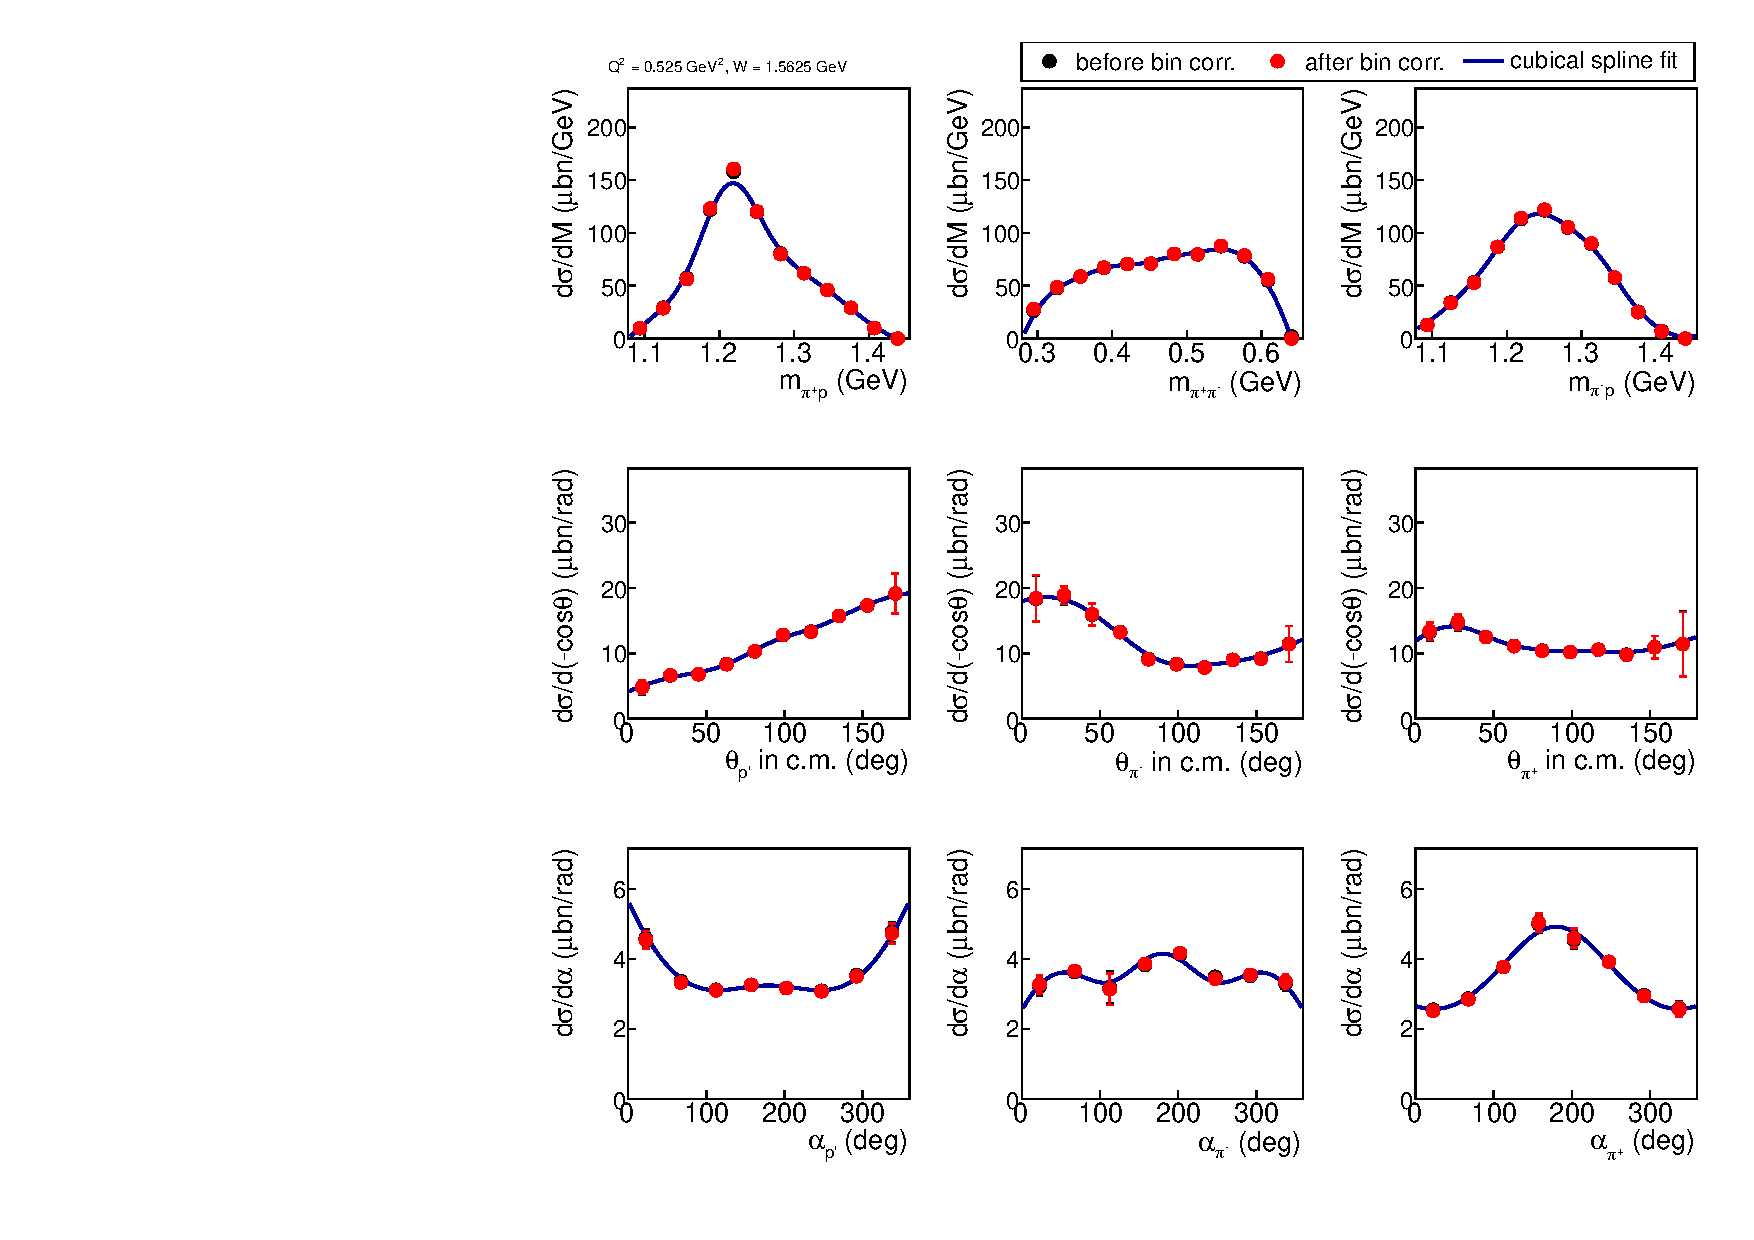
\includegraphics[width=10cm]{pictures/bin_corr/bin_corr_1d.pdf}
\caption{\small The single-differential cross sections as functions of the final hadron variables for one particular bin in $W$ and $Q^{2}$ ($W = 1.5625$~GeV, $Q^{2} = 0.525$~GeV$^{2}$) before  (black points) and after (red points) the binning corrections. Curves stand for the cubical spline approximation.} \label{fig:bincor_1d}
\end{center}
\end{figure}

\begin{figure}[htp]
\begin{center}
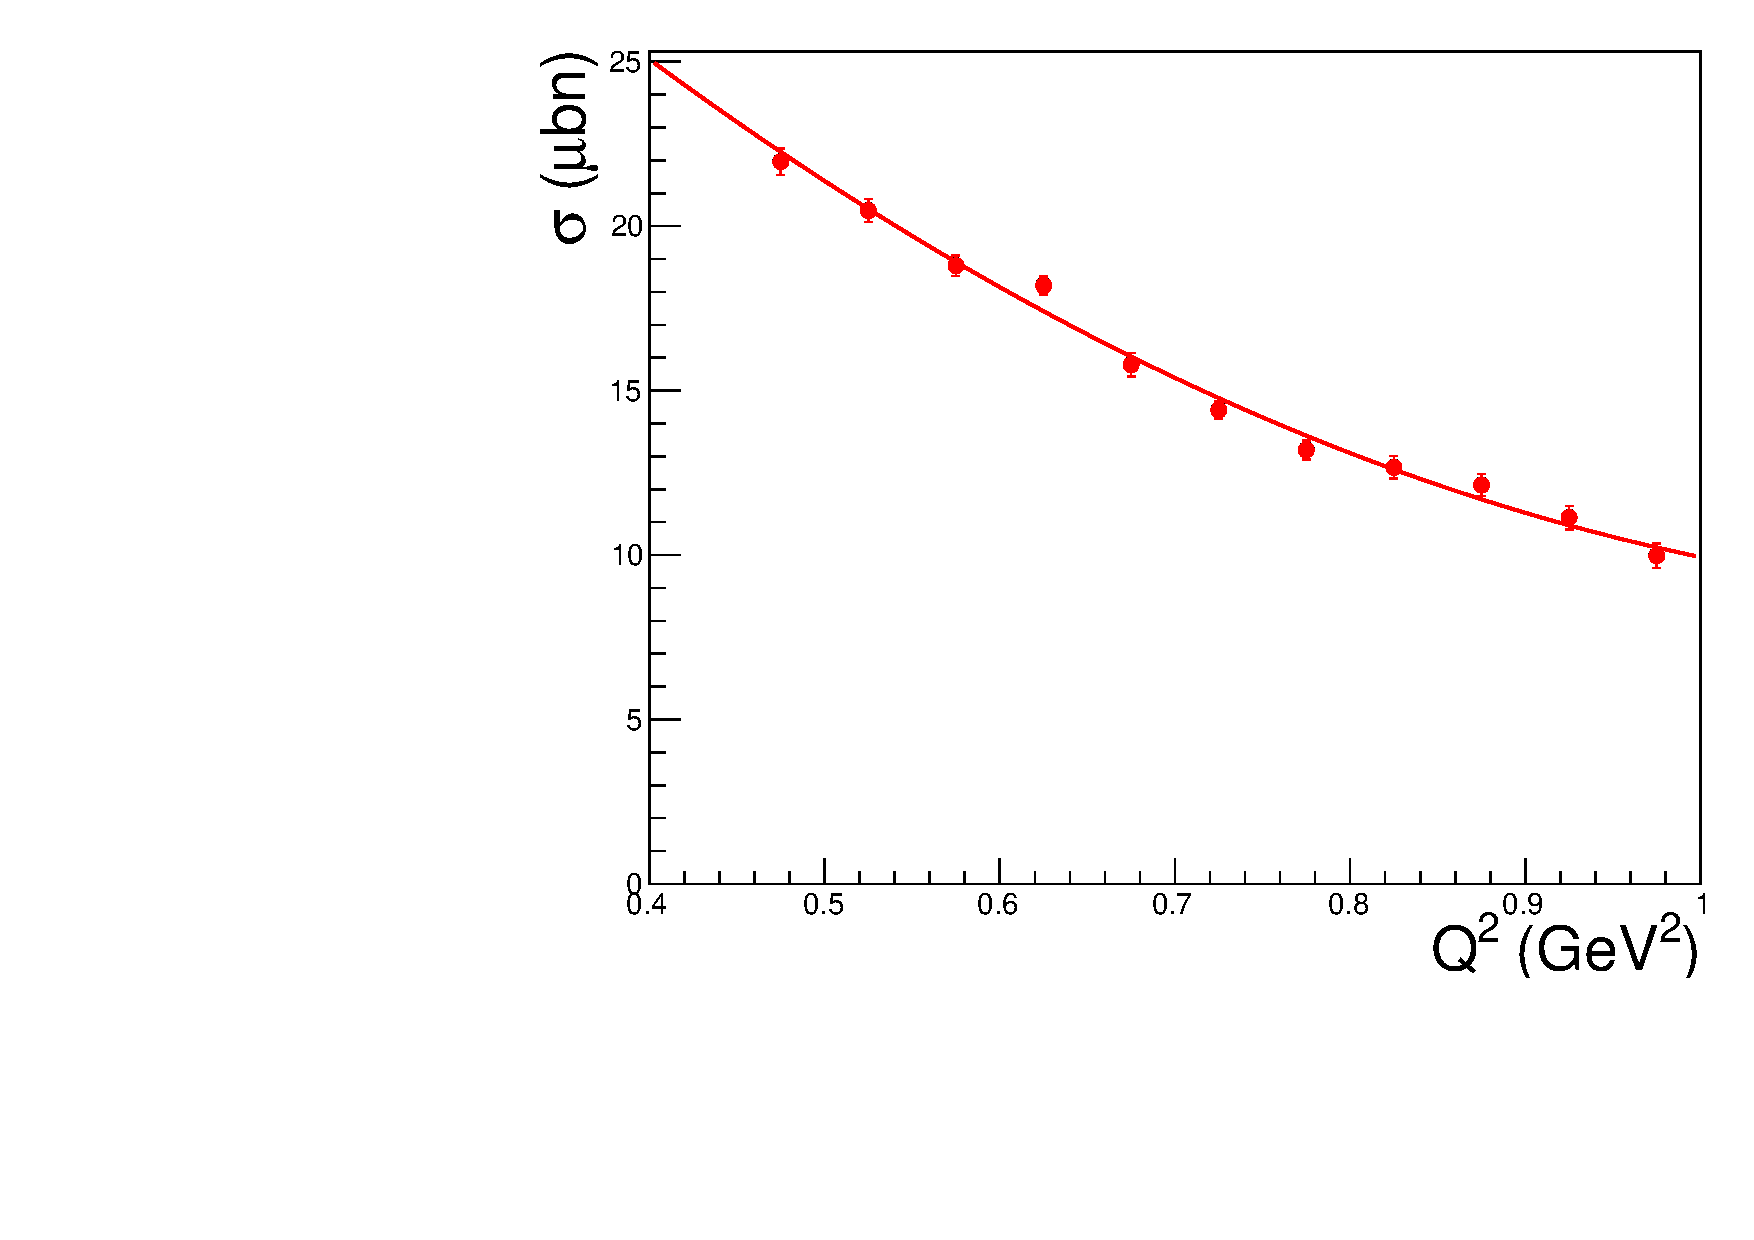
\includegraphics[width=7cm]{pictures/bin_corr/q2_fit.pdf}
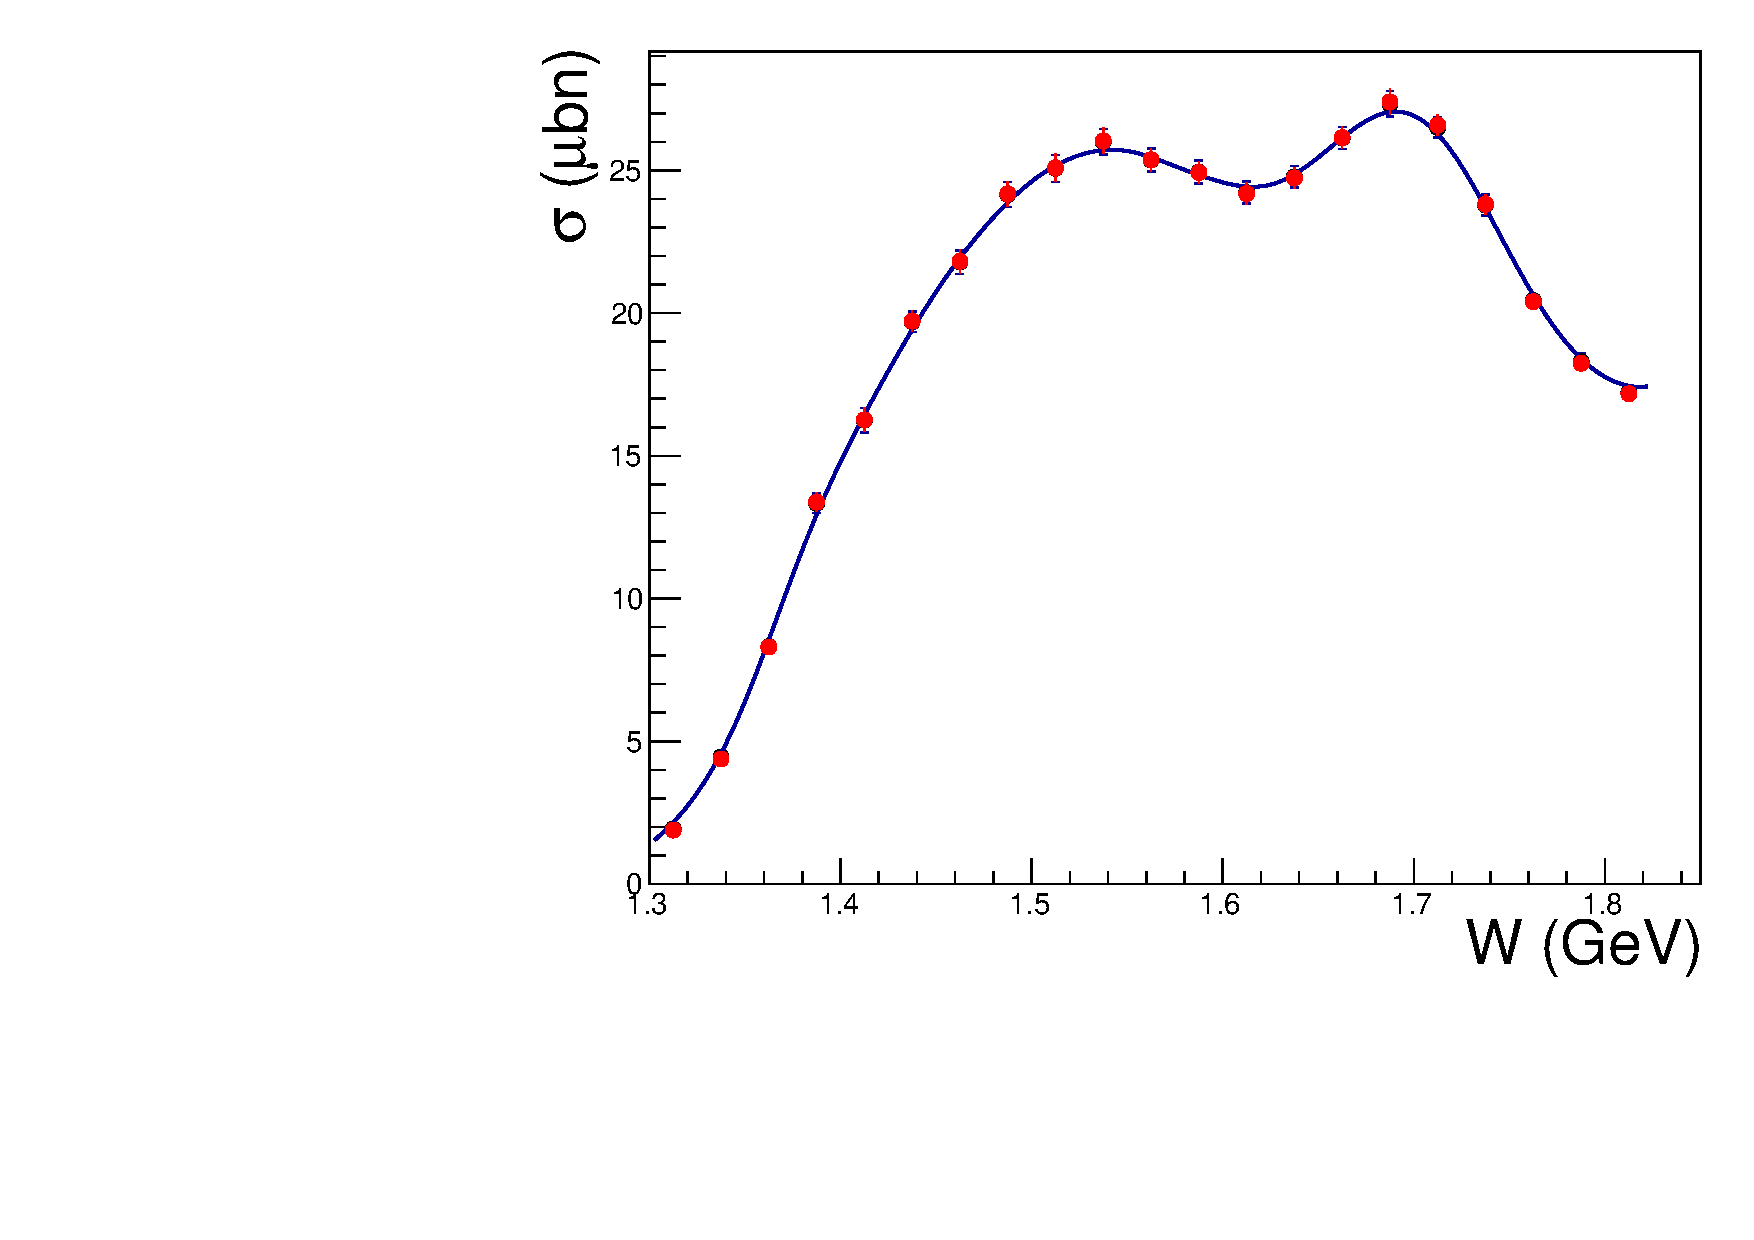
\includegraphics[width=7cm]{pictures/bin_corr/w_spline.pdf}
\caption{\small $Q^{2}$ dependence of integral cross section at $W = 1.4625$~GeV (left plot) and $W$ dependence of integral cross section at $Q^{2} = 0.475$~GeV$^{2}$ (right plot). On both plots black and red points correspond to the cross sections before and after the binning corrections, respectively. The curve on the left plot represents the second order polinomial fit, while the curve on the right plot correspond to the cubical spline approximation.} \label{fig:bincor_w_q2}
\end{center}
\end{figure}

Since in this analysis the detailed binning over all kinematical variables is chosen, the effect of the binning correction is rather small ($\sim 1\%$) and only in some points at low $W$ it can rise up to 4\%. That is why in the Figs.~\ref{fig:bincor_1d} and ~\ref{fig:bincor_w_q2} the black points (before the correction) are almost completely covered up by the red ones (after the correction).
